\begin{figure}[!b]
\centering
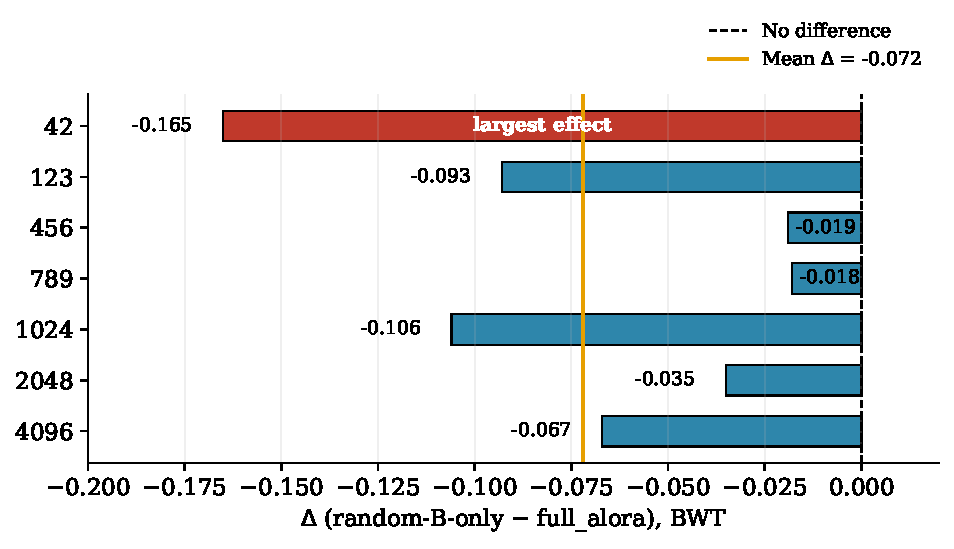
\includegraphics[width=0.55\textwidth]{figures/fig_forest_plot.pdf}
\caption{Per-seed within-\texttt{lora\_B} differences ($\Delta = \text{Random-B} - \text{Grad-Full}$, loss-based BWT, 7 seeds). All seven are negative (Random-B forgets less), mean $\Delta = -0.072$ (orange line); seed 42 is the largest effect ($-0.165$). Leave-one-out excluding seed 42 remains significant (paired $t(5)$, $p = 0.015$).}
\label{fig:forest}
\end{figure}

\begin{table}[!t]
\caption{\textbf{Headline result (D1, density-matched).} Both arms select the same 1{,}651{,}508 parameters (10\% of \texttt{lora\_B}); only the criterion differs. Per-seed loss-based BWT and $\Delta = \text{Random-B} - \text{Grad-B}$ (negative = random-B forgets less), seven sessions, one seed each. The last column is the density-\emph{unmatched} contrast from the same sessions, that is, Random-B against the unrestricted gradient mask ($\Delta = \text{Random-B} - \text{Grad-Full}$) rather than against Grad-B.}
\label{tab:d1}
\centering
\small
\begin{tabular}{@{}lccrr@{}}
\toprule
\textbf{Seed} & \textbf{Random-B BWT $\downarrow$} & \textbf{Gradient-B BWT $\downarrow$} & \textbf{$\Delta$ (matched)} & \textbf{$\Delta$ (unmatched)} \\
\midrule
42  & $\mathbf{0.278}$ & 0.453 & $-0.175$ & $-0.220$ \\
123 & $\mathbf{0.264}$ & 0.453 & $-0.188$ & $-0.119$ \\
456 & $\mathbf{0.283}$ & 0.406 & $-0.123$ & $-0.131$ \\
789 & $\mathbf{0.352}$ & 0.387 & $-0.035$ & $-0.074$ \\
1024 & $\mathbf{0.352}$ & 0.474 & $-0.121$ & $-0.109$ \\
2048 & $\mathbf{0.231}$ & 0.491 & $-0.261$ & $-0.187$ \\
4096 & $\mathbf{0.295}$ & 0.478 & $-0.183$ & $-0.166$ \\
\midrule
Mean & $\mathbf{0.294}$ & 0.449 & $-0.155$ & $-0.144$ \\
\bottomrule
\end{tabular}
\end{table}


\section{Experiments and Main Results}
\label{sec:experiments}

\subsection{Confounded and Density-Matched Comparisons}
\label{sec:confounded}


A first comparison follows the usual design, in which each method draws from its own pool. Under that design gradient attribution shows no advantage: its loss-based BWT is $0.437 \pm 0.061$ against $0.428 \pm 0.019$ for a shared random mask over five seeds, a seed-dependent difference that is not significant (Table~\ref{tab:cl_3b}, Appendix~\ref{app:null_stats}). Both methods still reduce forgetting relative to an unmasked adapter, but the comparison is uninformative about the selection rule, for the reason set out in \S\ref{sec:b0}: gradient attribution selects only \texttt{lora\_B} while the random baseline draws from both pools, so the design varies pool and criterion together. The result is reported for completeness and is distinct from the seven-seed comparison that follows, the two coming from different sessions whose absolute levels are not comparable (Appendix~\ref{app:nf4_drift}).



Holding the pool fixed changes the picture. We introduce a Random-B control drawn from \texttt{lora\_B} alone, matching the gradient mask's pool, and compare it against a gradient mask restricted to the same pool. Each seed is an independent session, so absolute BWT values drift between runs (Appendix~\ref{app:nf4_drift}) and only within-session paired observations are used. This comparison is matched on pool but not on density, since the gradient mask activates nearly twice as many \texttt{lora\_B} coordinates as Random-B. Even so, the random mask achieves the lower loss-based BWT in all seven seeds, with a mean difference of $-0.072$ that survives dropping the largest-effect seed (two-sided paired $t(5)=-3.62$, $p = 0.015$; Figure~\ref{fig:forest}, Appendix~\ref{app:within_b}). This value is the direct recomputation on the six retained paired contrasts and corrects the $p=0.029$ value reported in an earlier draft. That the direction is unchanged when the pool is fixed is the first indication that the criterion, rather than the pool, is what the earlier comparison was measuring.



\subsection{Density-Matched Control}
\label{sec:d1}

Pool and criterion are separated cleanly only when density is matched as well. The comparison above leaves the gradient arm activating about 20\% of the pool against 10\% for Random-B, so the two arms still differ in how many coordinates they train. D1 removes that difference, with both arms drawing exactly 10\% of \texttt{lora\_B} and only the ranking rule differing. At matched density the random mask again achieves the lower loss-based BWT in every seed, by a larger margin than in the density-unmatched comparison (Table~\ref{tab:d1}). Under a common [Grad-B $-$ Random-B] convention, the mean contrast is $+0.155$ on the V100 stack and $+0.152$ on the A800 stack. Thus the contrast reproduces at a similar magnitude in a second hardware/software environment; in a separate three-seed sensitivity check, reversing the execution order of the two arms does not reverse the Random-B--Grad-B contrast (Appendix~\ref{app:nf4_drift}).


\subsection{Task-Level Decomposition}
\label{sec:decomposition}

\begin{figure}[!htbp]
\centering
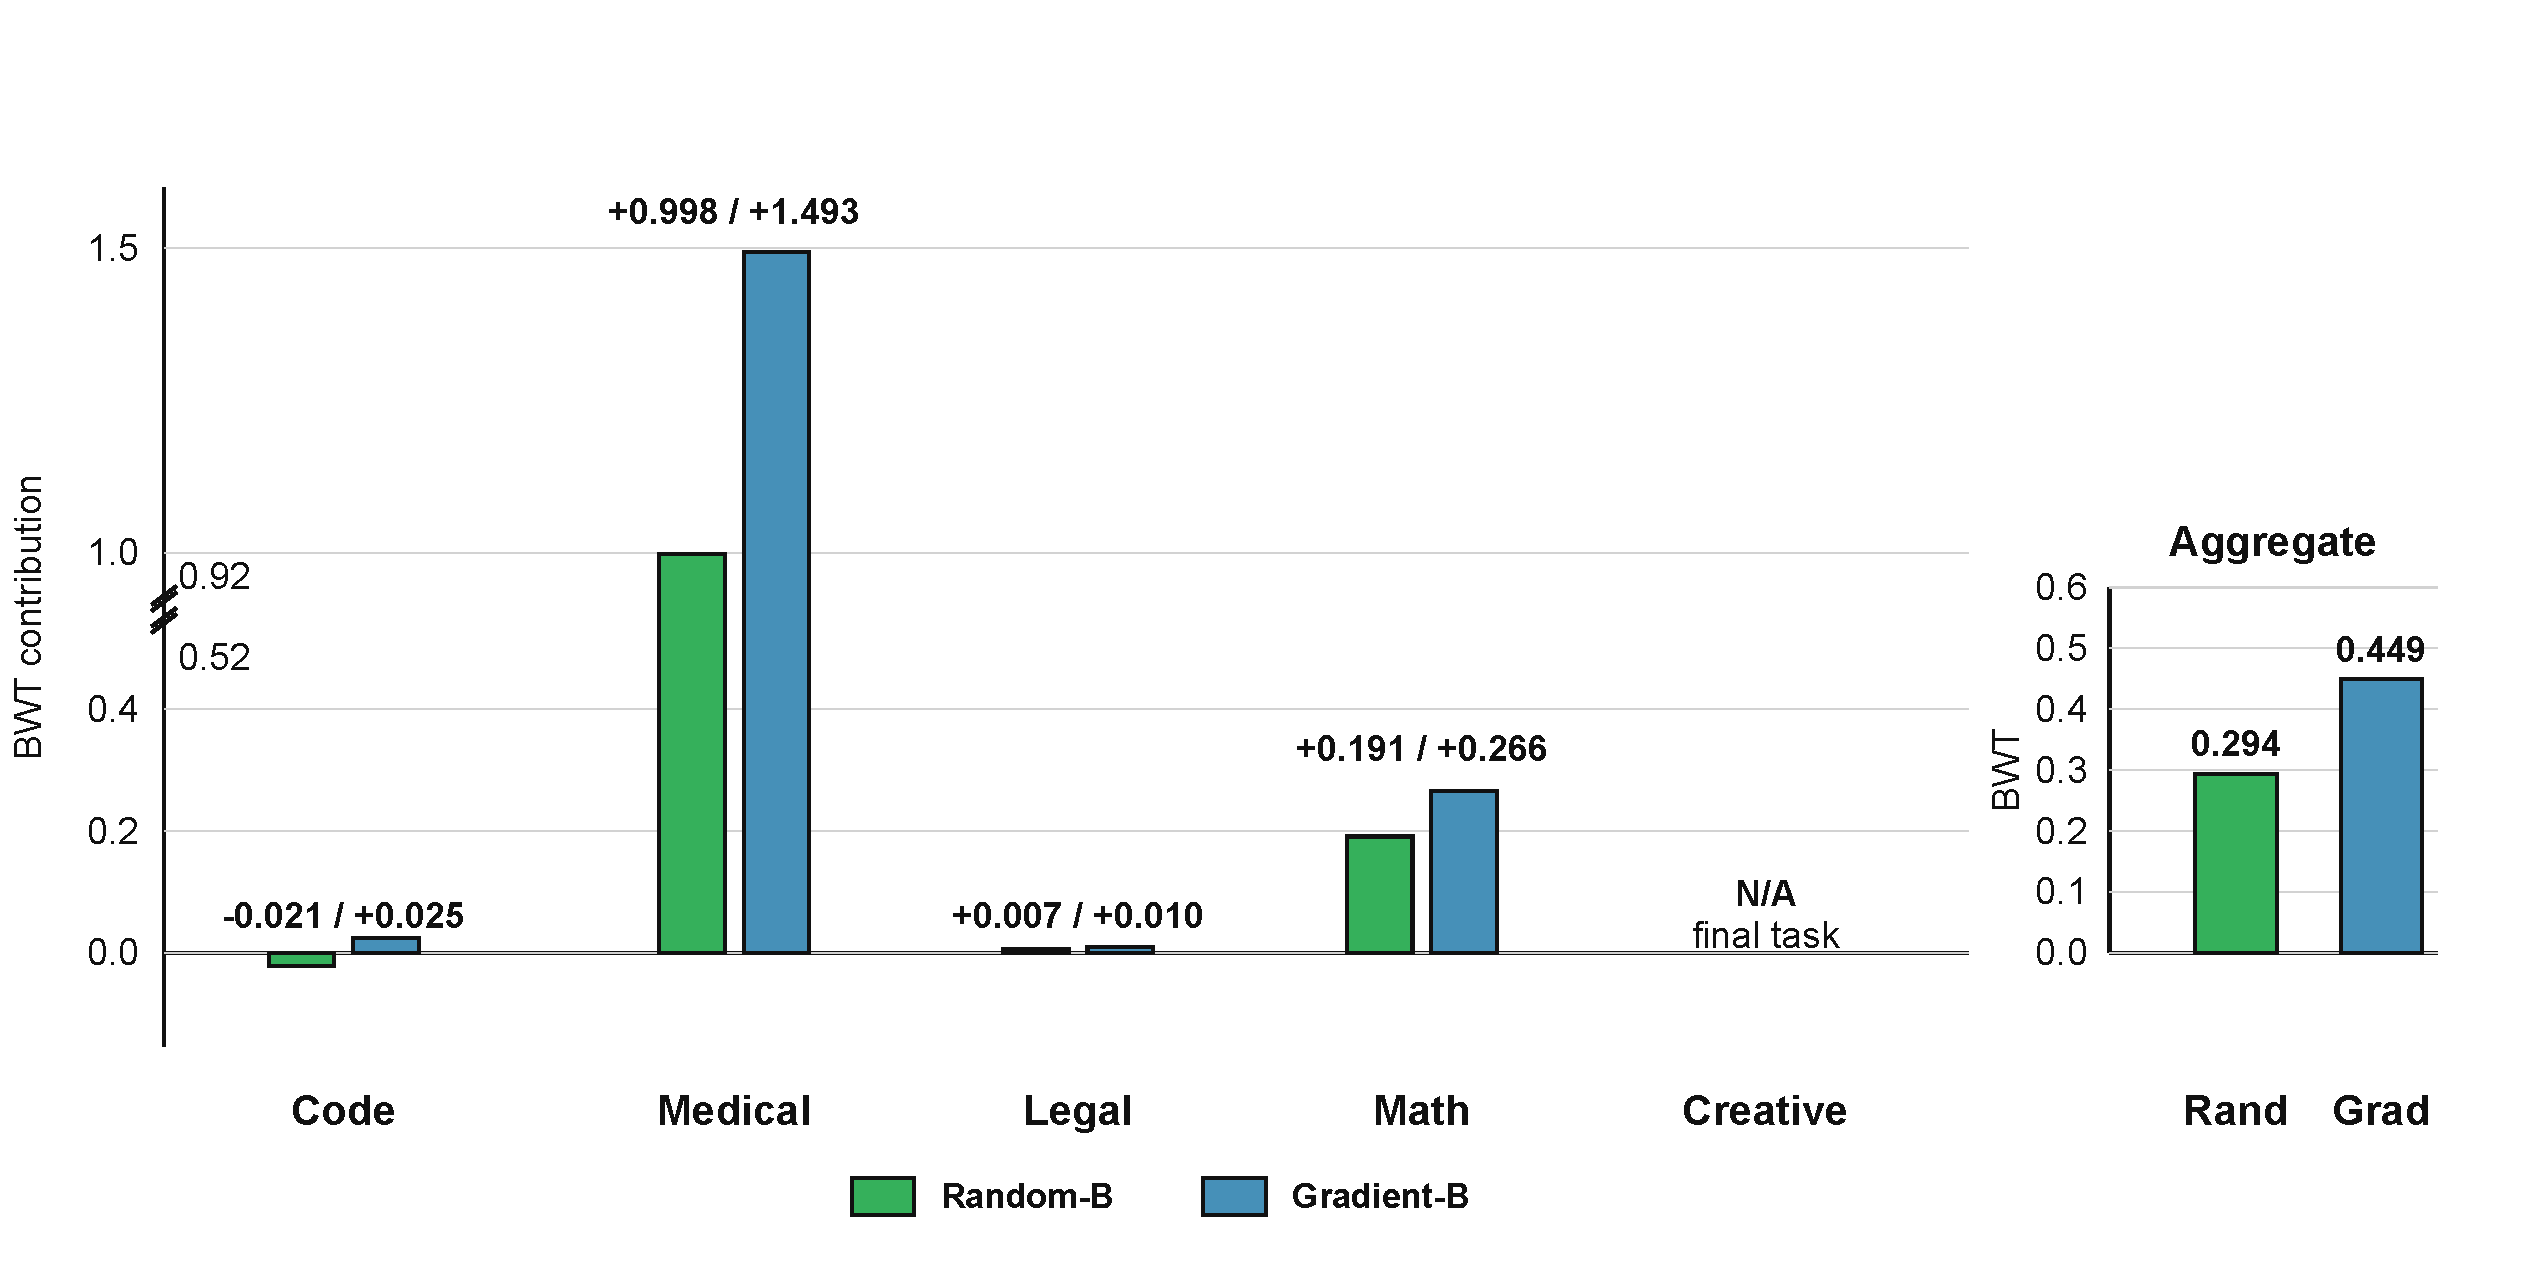
\includegraphics[width=0.9\textwidth]{figures/fig_d1_per_task_task_order_v8.pdf}
% \caption{D1 per-task decomposition, seven-seed means. Each task shows its Random-B (green) and Grad-B (blue) loss-based BWT contribution; the label above each task gives those two values in the same order. The per-task contributions span roughly two orders of magnitude, so the three small-magnitude tasks (Code, Legal, Math) share the lower segment of a broken y-axis while Medical is carried in the upper segment; the pair of slashes on each spine marks the omitted band, and the shared zero line runs unbroken across both segments. The right panel repeats the aggregate, a different quantity, on its own scale, drawn with its zero line on the same baseline. Random-B is lower on every task, with the effect concentrated on Medical; the per-seed table is in Appendix~\ref{app:d1_per_task}.}
\caption{The density-matched D1 per-task decomposition, averaged over seven seeds.
For each prior task, the bars show the loss-based BWT contribution of
Random-B and Grad-B, with the corresponding values
reported above each pair. 
Because the task-level contributions span roughly two orders of magnitude, the left panel uses a broken $y$-axis: the slashes mark the omitted interval from 0.52 to 0.92, and the labels above the Medical bars report their full values ($+0.998$ and $+1.493$) rather than truncated heights.
Creative is the final task and therefore has no backward-transfer contribution. The right panel shows
the aggregate loss-based BWT on a separate scale. Random-B exhibits less loss-based
forgetting on Code, Medical, and Math; the Legal difference is negligible and changes
sign across seeds. Most of the aggregate difference is concentrated on Medical.
Per-seed results are reported in Appendix~\ref{app:d1_per_task}.
}
\label{fig:per_task}
\end{figure}

The aggregate gain is not spread evenly across the five tasks, and where it concentrates bears on how the effect should be read. Medical carries about four fifths of it, while code and math contribute the remainder in the same direction; on legal the arms are indistinguishable. 
% Removing the medical task leaves the matched contrast at a little over a quarter of its headline size and still negative in every seed. 
% The three-task test is directional only, and the seven-seed test carries the significance claim (Appendix~\ref{app:d1_per_task}).
Two explanations can be assessed from the same data. First, the gradient arm's loss on each task's own diagonal is lower than the random arm's in every seed and task, yet it subsequently forgets more, so the two arms differ in retention rather than initial learning capacity. The same seven within-session pairs also show lower mean final held-out loss over the four prior tasks for Random-B: the Grad-B minus Random-B endpoint difference is $+0.0813$ (paired $t(6)=3.03$, $p=0.023$; 6/7 seeds). This endpoint result is less robust to leave-one-out deletion than the headline BWT contrast, but it shows that the effect is not merely a BWT normalization artifact (Appendix~\ref{app:d1_diagonal}). By contrast, restoring the gradient arm's full budget produces seed-dependent results: at seed 42 the density-matched gradient arm outperforms the unrestricted one, whereas the ordering reverses at the seven-seed mean. It therefore does not provide a stable explanation of the headline effect.

\subsection{Accuracy-Based Validation}
\label{sec:accuracy_branch}

% Loss-based BWT is a proxy for forgetting rather than the quantity of ultimate interest, so we evaluate the same masking comparison on task accuracy and ask whether the accuracy ordering agrees with the loss ordering. The evaluation reuses the primary protocol and the corrected task evaluators over the same seven seeds and 100 evaluation items per task, retraining from the base model on an A800 rather than re-scoring a saved checkpoint. Accuracy is scored only for the two tasks whose answers are discrete options (Medical, MedQA four options; Legal, CaseHOLD), so every quantity below concerns those two.

% The two masks are indistinguishable on accuracy: across seven seeds their difference averages $+0.94$ percentage points with a 95\% interval of $[-2.91, +4.80]$ that spans zero. A non-inferiority margin of 4 percentage points was specified in advance for this interval, and the measured upper bound exceeds it, so that criterion is not met. On the loss side the same masks are separated, with the gradient mask forgetting more in all seven seeds by a mean of $+0.152$; measured a second time on the A800 under a different implementation with the loss metric defined identically, the two estimates agree in magnitude to $0.003$ once the sign convention is aligned (the V100 figure is reported as [Random $-$ Grad] and the A800 figure as [Grad $-$ Random]; both describe the same contrast). Loss therefore resolves a difference the accuracy measurement does not, and the accuracy interval bounds that difference rather than contradicting it (Figure~\ref{fig:accuracy_ci}; per-seed values and the interval construction in Appendix~\ref{app:accuracy_seeds}).

\begin{figure}[!htbp]
\centering
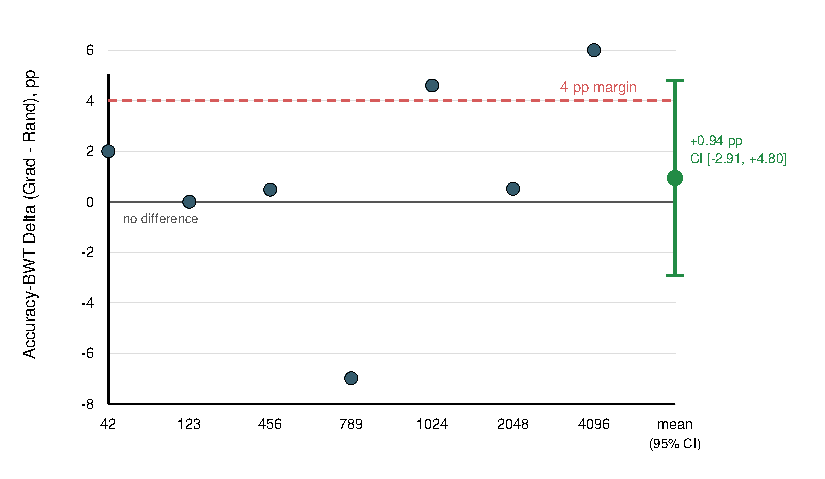
\includegraphics[width=0.6\textwidth]{figures/fig_accuracy_ci.pdf}
\caption{Accuracy-based validation. Blue points are the seven per-seed accuracy-BWT differences (Grad-B minus Random-B, percentage points) on the two discrete-option tasks, spanning $-6.98$ to $+6.00$ pp; green is the seven-seed mean with its 95\% interval $[-2.91,+4.80]$ pp. The plotted quantity is a difference of accuracy-BWT (mean final-minus-learned accuracy over prior tasks), a retention measure, not a difference of final accuracies. The interval spans zero, so no statistically reliable accuracy difference is detected, and it reaches past the 4 pp non-inferiority margin, so that criterion is not met. Per-seed values are in Appendix~\ref{app:accuracy_seeds}.}
\label{fig:accuracy_ci}
\end{figure}

Loss-based BWT is a proxy for forgetting rather than the quantity of ultimate interest, so we evaluate
the same masking comparison on task accuracy and ask whether the accuracy ordering agrees with
the loss ordering. The evaluation reuses the primary protocol and the corrected task evaluators over
the same seven seeds and 100 evaluation items per task, retraining from the base model on an A800
rather than re-scoring a checkpoint. Accuracy is scored only for the two tasks with discrete options
(Medical, MedQA four options; Legal, CaseHOLD), so every quantity below concerns those two.

Across seven seeds, the accuracy-BWT difference averages $+0.94$ percentage points with a
95\% interval of $[-2.91,+4.80]$ pp that spans zero. Here accuracy-BWT is the mean
final-minus-learned accuracy over the prior discrete-option tasks, so it measures retention on the
same footing as loss-based BWT and is not a difference of final accuracies. The individual seeds
range from $-6.98$ to $+6.00$ pp, and it is that spread rather than a large mean that makes the
interval wide at $n=7$. A 4 pp non-inferiority margin was specified in advance, and the measured
upper bound exceeds it, so non-inferiority is not established.

On the loss side, the same masks are separated: Grad-B forgets more in all seven seeds by a mean
of $+0.152$ on the A800 loss runs. This agrees in mean to within $0.003$ with the V100 estimate
after aligning sign conventions ($+0.155$ under [Grad $-$ Random]). Loss therefore resolves a
difference the accuracy measurement does not; the accuracy interval bounds that difference rather
than contradicting it.

Per-seed values and the interval construction are reported in Appendix~\ref{app:accuracy_seeds}.
Math is excluded from the accuracy read-out because its generation-based score is confounded by
truncation (Appendix~\ref{app:math_audit}).


